\section{Theory}
\label{sec:theory}

\subsection{introduction}

Within this experiment we try to monitor the absorption spectrum of Rubidium with a diode laser.
Therefor at first the functionality of diodes and lasers in general is explained.
By means of this we are able to present an accurate description of the diode laser and how to
use it for obtaining fluorescence.
Furthermore we will shortly treat the procedure and the whole setup of this experiment, including
the use of a diffraction grating and a piezo crystall.
At the end of this report we provide our results and discuss them.

\subsection{Functionality of a laser}
\label{sec:laser}

To start with explaining the functionality of a laser in general one may execute its abbreviation: "\textbf{L}ight \textbf{A}mplification by \textbf{S}timulated \textbf{E}mission of \textbf{R}adiation".
Because these arranged words are not enough to cover the complexity of a laser we present a more detailed
description in the following.

In general one needs four main components to realize a laser: a laser medium, a pump, a cooling system and a resonator.
The laser medium serves as a light source, when excited by the pump.
In order that the laser operates well, the medium has to consist of a material, where a so called population
inversion can be archieved by external excitation. To understand how this works, one may at first consider a
simple system with two energy levels. According to the Boltzmann statistics, the ground state is more occupied
than the excited state at finite temperature. Setting on an external pumping one may lift electrons from the
ground to the excited state. Because of spontaneous and induced emissions electrons will also fall back
to the ground state. Regarding this one is at most able to reach a population of $\SI{50}{\percent}$ in the excited
state. That means, however, that a population inversion, which is required for a well working laser, cannot be
produced by a two level system. Hence we now pay attention to a three level system like the one depicted in
illustration \ref{fig:threelevelsystem}.
\begin{figure}
  \centering
  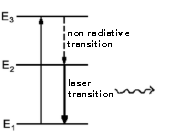
\includegraphics[height = 4.3cm]{Ordnername/threelevel_edit.pdf}
  \caption{Schematic plot of the three level system that can be used in a laser medium \cite{threelevel} \textit{edited}.}
  \label{fig:threelevelsystem}
\end{figure}
Via external pumping the electrons can be lifted to a third energy level, which lies energetically above the second one.
Furthermore electrons from the third level transit non radiative to the second level. Again the laser transition is
caused by electrons falling back from the second to the first state, but in contrast to the two level system they
don't transit via induced emissions caused by the external pumping. The reason for this lies in the fact,
that incoming photons can only induce energy transitions,
when the energy difference between the involved states equals the photon energy. However, the external pumping
in our considered three level system induces already absorptions from the first to the third state
($\Delta E = E_3 - E_1$) and therefor cannot induce emissions from the second to the first
state ($\Delta E = E_2 - E_1$). Because the induced emissions by the external pumping omit, one may realize
that the laser transitons occur rarely compared to those within the two level system. It can be shown,
that a population inversion between the first and the second state can be archieved if the
spontaneous non radiative transitions from state three to state two happen much more frequently than the
spontaneous emissions from state two to state one. Thus a medium with a three level system
appears to be sufficient for using it as a laser medium.

However, there are several different possibilities, to excite the laser medium external, for instance thermal pumping,
electrical pumping, which is used in this experiment, or even chemical pumping.
In none of these cases it is possible to convert the full amount of energy, which is pumped into the system, to
radiation. A non negligible part is transfered to phonons and therefor resulting in heat.
Using a cooling system will guarantee for a constant temperature of the laser medium, so that the thermal radiation
stays constant and the laser doesn't overheat.

At this point we remind the reader that the spontaneous emitted photons are,
in opposition to the external pumping photons, able to induce emissions from the second to the first level,
because they have exactly the required energy. This is precisely what is made use of inside a laser with help
of a resonator as can be seen in Fig. \ref{fig:lasersetup}. The spontaneous emitted photons of the
laser transition radiate to the partly reflecting front- and the fully reflecting backside of the laser can.
After the light is reflected, it radiates back into the laser medium and induces laser transitions as mentioned above.
The two parallel mirrors also form a resonator for the arising light beam:
Light modes with certain frequencies are amplified because they enjoy constructive interference while others
are weakened because of destructive interference. The difference between the frequencies of two next neighbour
constructive modes is called free spectral range and given by
\begin{align}
  \Delta \nu_\text{FSR} = \frac{\text{c}}{2 L n},
  \label{eqn:freespectralrange}
\end{align}
where $c$ is the speed of light, $L$ is the length of the resonator and $n$ is the refraction index of the
laser medium.

\begin{figure}
  \centering
  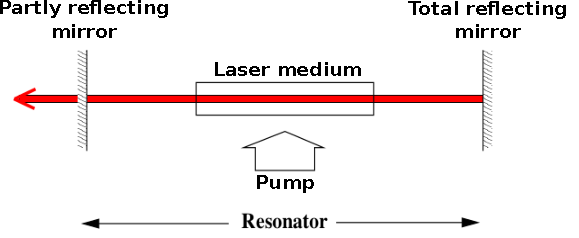
\includegraphics[height = 4.0cm]{Ordnername/lasersetup_edit.pdf}
  \caption{Setup of a laser in principle \cite{manual2} \textit{edited}.}
  \label{fig:lasersetup}
\end{figure}

With all the mentioned components of the laser setup one is able to generate an almost monochromatic and coherent laser beam.
To improve the laser with regard to its frequency width it is e.g. possible to build an external cavity with a diffraction
grating. We will treat this later.

The main property of a diode laser is that it contains a semiconductor medium and an electrical current pump forming a diode.
Thus we present a short description of semiconductors, doping of them and the funcionality of a diode in the following sections.

\subsection{Semiconductors and doping}

A semiconductor is a material with two main properties: it conducts weaker than a metall, but stronger than an insulator and
its conductivity rises with the temperature. The illustrative reason for the enumerated things is, that the Fermi energy of
those materials is located inside a narrow band gap of the band structure. That means, that at zero temperature the valence band of a semiconductor is
filled, while the conducting band is empty, so no current can occur. At higher temperatures thermal excitations let the electrons overcome
the band gap, so that the conductivity increases.

Doping a semiconductor means placing impurities into it to change its conductivity substantial.
One distinguishes between doping with donor materials and doping with acceptor materials.
In the first case the impurity provides an additional electron, which is energetically by far closer to the
conductive band than the valence band. The consequence is, that the conductivity increases, because
the additional electrons only needs to overcome a smaller band gap. In the second case the impurity
provides a hole, which lies energetically near to the valence band. This hole can be occupied by an electron
with much less energy than in the non doped case, so that the conductivity again rises.
Both concepts are illustrated in Fig. \ref{fig:donor} and \ref{fig:acceptor}.

\begin{figure}
  \centering
  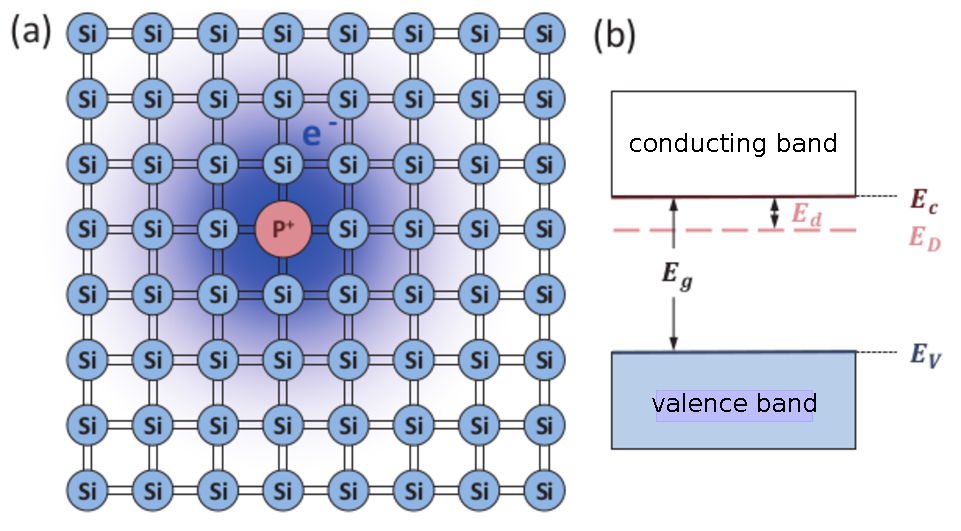
\includegraphics[height=5cm]{Ordnername/donor_edit.pdf}
  \caption{(a) Illustration of the grid of n-doped silicon. The phosphor impurity serves as an electron donor.
  (b) Schematic depiction of the band structure of a n-doped semiconductor \cite{semiconductors} \textit{edited}.}
  \label{fig:donor}
\end{figure}

\begin{figure}
  \centering
  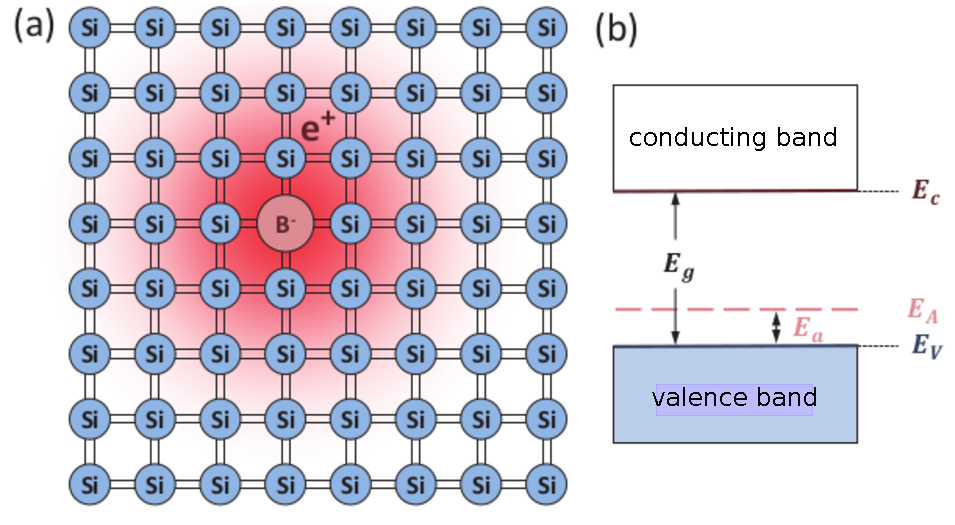
\includegraphics[height=5cm]{Ordnername/acceptor_edit.pdf}
  \caption{(a) Illustration of the grid of p-doped silicon. The boron impurity serves as an electron acceptor.
  (b) Schematic depiction of the band structure of a p-doped semiconductor \cite{semiconductors} \textit{edited}.}
  \label{fig:acceptor}
\end{figure}

\subsection{Funcionality of a diode}

Basically a diode consists of a semiconductor material, which is p-doped on one side and n-doped on the other side.
Without any external influences some of the almost not bounded electrons from the n-doped side will recombine, among emission of a photon,
with some holes from the p-doped side, caused by diffusion. The result is firstly a transition zone between the two doped sides, where
no free charge carriers remain, and secondly an electric field, which acts against the progress of recombination,
because it accelerates electrons from the p-doped side to the n-doped side. After a short time the system arrives at an equilibrium state,
where the diffusion current and the counter field current vanish. The width of the so called depletion zone at this point
depends on the doping densities and the diffusion potential.

However, if one attaches a power supply to the presented configuration, meaning to the diode, there are two relevant cases to consider:
In the first case the plus terminal is connected to the n-doped side, while the minus terminal is connected to the
p-doped side. The consequence is, that the doped semiconductor loses its conductivity, because the depletion layer width
increases as the remaining free charge carriers are pulled out by the power supply. One calls this configuration of the diode
the reverse or blocking direction. The second case includes connecting the poles the other way round, so that of course
the depletion layer width decreases and the conductivity rises. This setting is called the forward or passing direction of the diode.
As a conclusion of this section the current-voltage characteristic of the diode is presented in Fig. \ref{fig:currvolt}

\begin{figure}
  \centering
  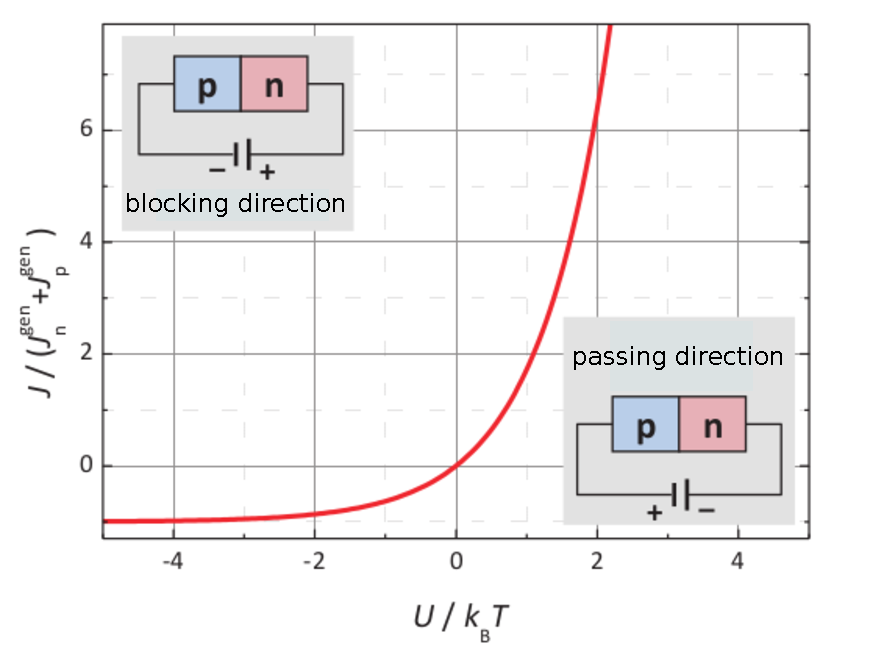
\includegraphics[height=6cm]{Ordnername/currvolt_edit.pdf}
  \caption{Current-voltage characteristic of the diode \cite{semiconductors} \textit{edited}.}
  \label{fig:currvolt}
\end{figure}

\subsection{Functionality of a diode laser}
\label{sec:funclaser}

To realize a diode laser, one has to operate with the diode in forward direction.
Electrons from the narrow depletion zone are pulled to the plus terminal, while
holes are pulled to the minus terminal. Because of diffusion, electrons and holes from the doped sides
recombine again in the depletion zone, while emitting a photon. Due to this, the depletion zone is
also called active layer. Its width stays constant within the permanent repetition of the enumerated
processes. So as a result of the pn-transition and the external electrical pumping one has a diode
with a light emitting active layer.

Because the active layer has a larger index of refraction than the surrounding layers, the emitted light is confined
and expands only within a tiny channel. To realize the resonator mentioned in section \ref{sec:laser} the front
and back facets of the semiconductor are cleaved to act as cavity mirrors. If the pump current lies under a
certain threshold, the stimulated gain is lower than the optical losses and the output of the diode laser is
comparable to that of a LED. Above this threshold the stimulated emission causes a population inversion and therefor
a strong light amplification. The intensity of the resulting coherent laser beam increases linearly with the current.

However, this is not the full necessary theoretical part of this experiment, because two problems occur:
The linewidth of the output beam is around $\Delta \nu \approx \SI{50}{\mega\hertz}$, so larger than the atomic transitions
of rubidium $\Delta \nu_\text{Rub} \approx \SI{5}{\mega\hertz}$ and the diode laser is very sensitive to optical feedback.
In the next section an optical instrument, which solves those problems, is presented.

\subsection{Optimizing the laser beam}
\label{sec:Optimizing}

A possible solution for the enumerated problems in the last section is presented in Fig. \ref{fig:diffraction}.
After the output beam is collimated by a lens it hits a diffraction grating. With this optical tool, the optical
feedback is not deactivated, but controlled. Most of the light, however, is reflected by the diffraction grating,
but around $\SI{15}{\percent}$ strays back into the diode. So the grating and the back facet of the diode form
an external cavity for the laser beam. The consequences of this are explained later.

\begin{figure}
  \centering
  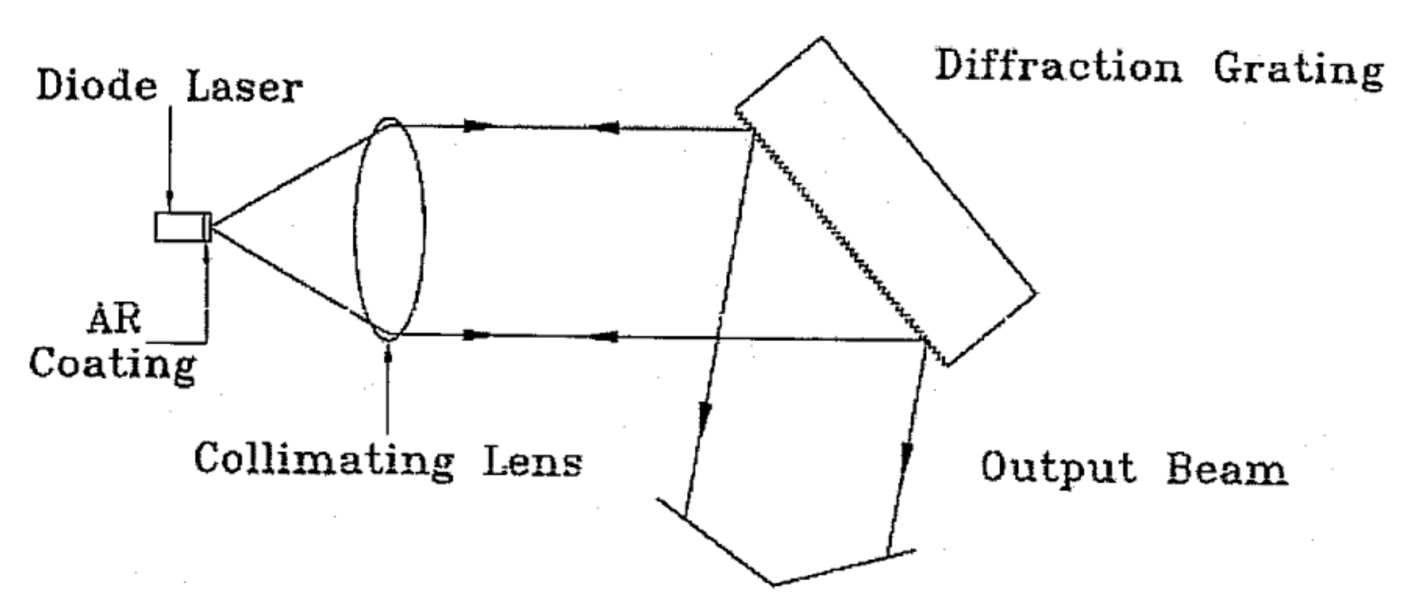
\includegraphics[height=5cm]{Ordnername/diffraction_edit.pdf}
  \caption{Setup of the diode laser with an external diffraction grating \cite{manual} \textit{edited}.}
  \label{fig:diffraction}
\end{figure}

Considering the total construction one has four different contributions to the optical gain of the laser:
the medium gain, the internal cavity, the grating feedback and the external cavity.
In Fig. \ref{fig:optgain} this is illustrated. Theoretically the laser will lase in the mode with the
highest net gain, because this mode amplifies itself the most via stimulated emission. In practice more
modes can occur at once and the output frequency can vary chaotically. One task in this experiment is to
estimate parameter configurations to get a single mode output through adjustment.

\begin{figure}
  \centering
  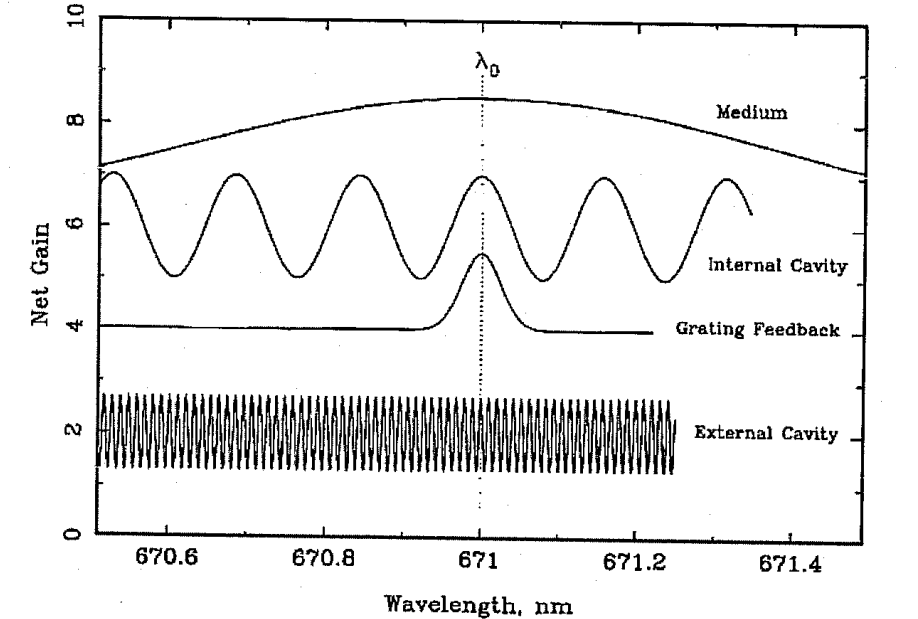
\includegraphics[height=7cm]{Ordnername/optgain.png}
  \caption{Schematic trend of the net gain for the four contributions \cite{manual}.}
  \label{fig:optgain}
\end{figure}

%One obtains that the wavelength increases almost linearly with the temperature.
The position of the maximum of the broad medium gain peak depends on the temperature of the laser.
After adjusting the temperature and therefor the wavelength to the required value, the medium gain can be neglected, because
of its broad peak.

Like mentioned before, the diode can forms an internal resonator or optical cavity, where frequently, as shown in equation
\eqref{eqn:freespectralrange}, certain wavelengths are amplified. The laser will tend to lase in those modes,
because the net gain is at the maximum. One can affect the wavelength by directly increasing the temperature of the
laser head, which is impractical, because it requires some time. However, the wavelength can also be manipulated, while
raising the pump current. The latter increases firstly the temperature very fast, within a time scale of about $\SI{1}{\micro\second}$,
and secondly the carrier concentration inside the active layer and hence the optical path length.
At this point we emphasize, that even though the temperature and therefor the wavelength can be varied, not every required
wavelength can be reached with adjusting the bare laser. Because of the oscillating internal cavity gain the wavelength shifts at
certain temperatures or current values and so called mode hops occur. This adds up to the two problems counted in section
\ref{sec:funclaser} and can be solved by the same optical tool: a diffraction grating.

The first presented contribution to the net gain by the diffraction grating is the grating feedback. The incoming light
is dispersed by the grating and a wavelength band with narrow width is emitted back into the laser. So the net gain
function consists of only one peak like one can view in Fig. \ref{fig:optgain}. Its position is determined by the horizontal grating angle,
and the grating itself, especially the space $d$ between the grating lines. The width of this peak depends on the
expansion of the laser beam and the amount of grating lines.

The second and last contribution to the net gain by the diffraction grating is the external cavity. One can recognize in Fig. \ref{fig:optgain},
that the resulting net gain function has a higher frequency than the net gain function of the internal cavity. This is constituted by
the depending of the free spectral range, see equation \eqref{eqn:freespectralrange}, on the reciprocal length of the resonator.
To comprehend the interaction of the contributions of the grating feedback, the internal and the external cavity one may have a
look at the so called best guess picture in Fig. \ref{fig:bestguess}. In the illustrated optimal case the laser will lase in the mode, where
the cavity and feedback contributions are at maximum, but this is of course not the general case.

\begin{figure}
  \centering
  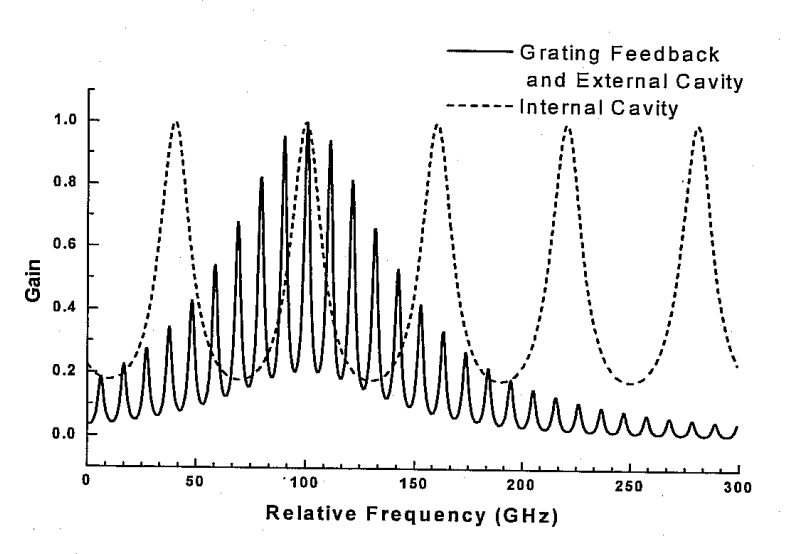
\includegraphics[height=7cm]{Ordnername/bestguess.png}
  \caption{Best guess picture of the internal, external and grating feedback contibutions to the net gain \cite{manual}.}
  \label{fig:bestguess}
\end{figure}

In general it results, that the broad band internal cavity modes dominate at the long scale frequencies, while the narrow band external cavity modes
dominate at the short scale frequencies. An instance for this is presented in illustration \ref{fig:continter}.
The net gain function of the grating feedback and the external cavity can be shifted continuously, when varying the
horizontal grating angle. As shown in Fig. \ref{fig:continter} \textbf{b},\textbf{c} the small changing
of the grating angle causes firstly a continuous shifting of the frequency and secondly, when a threshold is reached, short scale
mode hops between the external cavity modes. When a certain threshold within the long scale is reached by adjusting the laser, a broad mode hop occurs
between the internal cavity modes, like shown in Fig. \ref{fig:continter} \textbf{d}.
As explained above the narrow band external cavity modes dominate at short scale frequencies, so if one only adjusts the grating angle, only
a narrow frequency band around the internal modes can be reached. This can also be noticed, when viewing Fig. \ref{fig:continter}.
The discussed thing seems to be a problem, but we remind the reader, that the internal modes can also be varied by changing the current.
Together the full frequency spectrum is covered continuously.

\begin{figure}
  \centering
  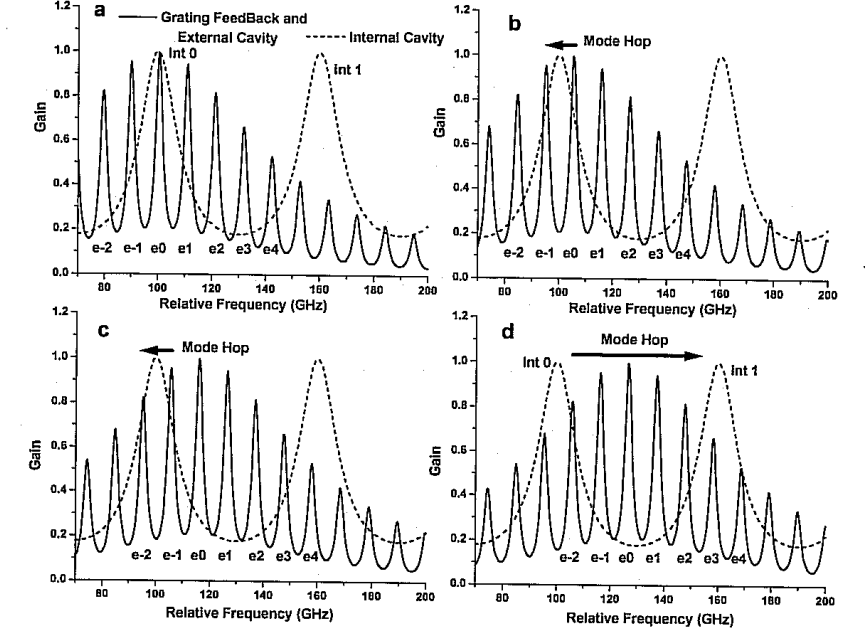
\includegraphics[height=10cm]{Ordnername/continter}
  \caption{An Instance to comprehend the short and long scale mode hops, that occur, when adjusting the grating angle.
  Fig. \textbf{a} shows the starting position, \textbf{b} and \textbf{c} show external cavity mode hops and in the
  last Fig. \textbf{d} one can see an internal cavity mode hop \cite{manual}.}
  \label{fig:continter}
\end{figure}

\subsection{Absorption spectrum of Rubidium}

The analysed Rubidium probe in this experiment consists of the isotopes $\ce{^{85}Rb}$ and $\ce{^{87}Rb}$.
In Fig. \ref{fig:dopplerandterm} one can view the relevant atomic hyperfine transitions, that can be induced
with the output wavelength of the diode laser. When the right wavelength is adjusted, the Rubidium cell
absorbs a big part of the light and emitts it in any direction, so that the intensity of the beam decreases
in the direction of expansion. This lack of intensity can be detected with a diode behind the Rubidium cell.
Even though the transition energies are very precise, even when regarding the energy unsharpness,
one obtains a relatively broad laser peak, because of the Doppler widening.
The Rubidium atoms can move almost freely inside the cell and therefor the wavelength obtained from their inertial system
is in general not equal to the one obtained in the labour system. As a result the absorption peak gets more broad, because atoms
moving towards the laser beam are excited by higher wavelengths, while atoms moving in the other direction are excited
by lower wavelengths. The Doppler broaden spectrum is also presented in Fig. \ref{fig:dopplerandterm}. How this can
be monitored within this experiment is shortly described in the procedure section.

\begin{figure}
  \centering
  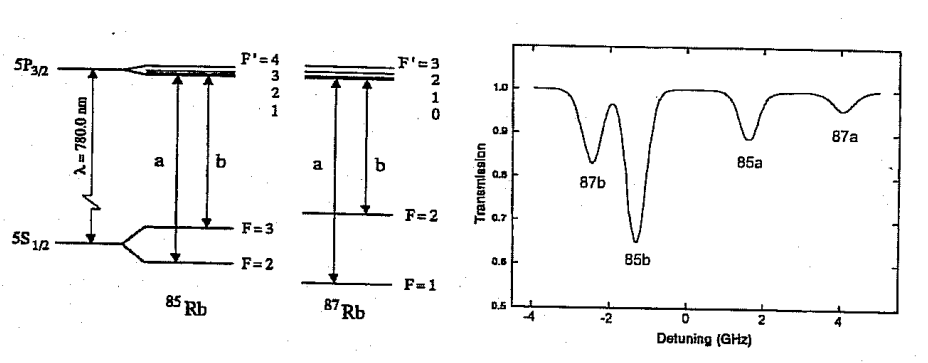
\includegraphics[height=5.8cm]{Ordnername/dopplerandterm.png}
  \caption{Left: Term scheme and relevant transitions. Right: Doppler broaden spectrum \cite{manual}.}
  \label{fig:dopplerandterm}
\end{figure}

\subsection{Piezo crystall}

The piezoelectrical effect comprises the mutual interaction between an external deformation and an
electrical potential inside a piezo crystal. It is used in this experiment, to vary the grating
position continuously, so that the required wavelengths to induce the rubidium transitions are runned through.
Therefor a piezo crystal is placed below the diffraction grating and connected to an alternating current.
Together with some other techniques presented in the following section one is able to obtain a
Doppler broaden spectrum like the one in Fig. \ref{fig:dopplerandterm}.
